% =====================================================================
% Análisis de complejidad por función — Proyecto 9: Coloreo de Grafos
% Grupo 10 · Análisis y Diseño de Algoritmos · UNMSM
% Compilar: pdflatex analisis_complejidad.tex  (dos pasadas), u Overleaf.
% =====================================================================
\documentclass[11pt,a4paper]{article}

\usepackage[utf8]{inputenc}
\usepackage[T1]{fontenc}
\usepackage[spanish,es-tabla,es-noshorthands]{babel}
\usepackage{lmodern}
\usepackage[margin=2.3cm]{geometry}
\usepackage{amsmath,amssymb,amsthm,mathtools}
\usepackage{booktabs,array}
\usepackage{xcolor}
\usepackage{listings}
\usepackage{graphicx}
\usepackage{enumitem}
\usepackage[hidelinks]{hyperref}

\definecolor{codegray}{gray}{0.45}
\definecolor{codeback}{gray}{0.965}
\lstset{
  language=Python, basicstyle=\ttfamily\small, numbers=left,
  numberstyle=\tiny\color{codegray}, numbersep=8pt, xleftmargin=2.2em,
  backgroundcolor=\color{codeback}, frame=single, framerule=0.2pt,
  keywordstyle=\bfseries, commentstyle=\color{codegray}\itshape,
  showstringspaces=false, columns=fullflexible, keepspaces=true,
  breaklines=true, tabsize=4, literate={í}{{\'i}}1 {á}{{\'a}}1 {é}{{\'e}}1
  {ó}{{\'o}}1 {ú}{{\'u}}1 {ñ}{{\~n}}1 {Δ}{{$\Delta$}}1 {Θ}{{$\Theta$}}1
}

\newtheorem{teorema}{Teorema}[section]
\newtheorem{lema}[teorema]{Lema}
\newtheorem{proposicion}[teorema]{Proposición}
\theoremstyle{definition}
\newtheorem{definicion}[teorema]{Definición}
\theoremstyle{remark}
\newtheorem{observacion}[teorema]{Observación}

\newcommand{\dg}{\operatorname{deg}}
\newcommand{\bigO}{\mathcal{O}}

\title{\textbf{Análisis de complejidad función por función}\\[2mm]
\large Proyecto 9 --- Asignación de frecuencias (FAP) mediante coloreo de grafos\\
Caso de estudio: mapa del Perú (25 departamentos)}
\author{Grupo 10 --- Análisis y Diseño de Algoritmos, UNMSM}
\date{Semestre 2026-I}

\begin{document}
\maketitle

\begin{abstract}
Se analiza, \emph{función por función}, la complejidad temporal y espacial del
código del Proyecto~9 (paquete \texttt{src/}). El método es uniforme: cada
función se \textbf{divide en bloques}, a cada línea se le asigna un costo
unitario $c_i$ y un número de ejecuciones $t_i$, el tiempo se plantea como la
\textbf{sumatoria} $T=\sum_i c_i t_i$ y esta se resuelve hasta una forma cerrada
que se acota asintóticamente. Se usan además: identidades combinatorias (lema
del apretón de manos), análisis amortizado (orden smallest-last, muestreo de
$G(n,p)$), conteo agregado con borrado perezoso (DSATUR), árboles de recursión
(backtracking) y esperanza matemática (generadores aleatorios). Se cubre el
coloreo por distancia (recorrido BFS desde el departamento elegido) usado por la
aplicación visual. El mapa, la adyacencia y los centroides se derivan de un
GeoJSON oficial de los 25 departamentos.
\end{abstract}

\tableofcontents
\newpage

% =====================================================================
\section{Metodología}\label{sec:metodo}
% =====================================================================

\subsection{Modelo de cómputo}
Se usa el modelo \textbf{RAM} con criterio de costo uniforme: cada operación
elemental cuesta una constante $c_i>0$. El tamaño de un grafo $G=(V,E)$ se
describe con $n=|V|$ y $m=|E|$; $\Delta(G)$ es el grado máximo y $\dg(v)$ el
grado de $v$.

\begin{observacion}[diccionarios y conjuntos]\label{obs:hash}
El grafo se representa con \texttt{dict} y \texttt{set} (tablas hash): inserción,
búsqueda y borrado cuestan $\bigO(1)$ \emph{en promedio}. Como las claves son
enteros que generamos nosotros (no adversariales), usamos ese costo promedio en
todo el documento; las cotas son, en rigor, esperadas.
\end{observacion}

\subsection{Método de bloques y sumatorias}\label{sec:bloques}
\begin{enumerate}[label=\textbf{Paso \arabic*.}, leftmargin=2.4cm]
\item \textbf{Dividir en bloques} $B_1,B_2,\dots$ (inicialización, bucle
  externo, bucle interno, retorno): un bloque es un fragmento cuyo número de
  repeticiones se describe con una sola expresión.
\item \textbf{Costo por línea}: costo unitario $c_i$ y repeticiones $t_i$. Una
  cabecera de bucle que itera $k$ veces aporta $t_i=k+1$; su cuerpo $t_i=k$.
\item \textbf{Plantear la sumatoria} $T(n,m)=\sum_i c_i\, t_i(n,m)$. Si el costo
  de una iteración depende del vértice (p.\,ej.\ $\dg(v)$), la sumatoria se
  escribe sobre los vértices.
\item \textbf{Resolver y acotar} hasta forma cerrada y concluir
  $T=\Theta(f)$ (o $\bigO$ cuando solo se acota por arriba).
\end{enumerate}

La identidad clave es el \emph{lema del apretón de manos}:
\begin{equation}\label{eq:handshake}
  \sum_{v\in V}\dg(v)=2m,
\end{equation}
pues cada arista aporta $1$ al grado de sus dos extremos. Por ello ``recorrer la
vecindad de cada vértice una vez'' cuesta $\Theta(n+2m)=\Theta(n+m)$: la firma de
los algoritmos lineales sobre grafos dispersos. Para funciones recursivas el
Paso~3 da una \emph{recurrencia} (se resuelve con árbol de recursión); para
costos irregulares, \emph{análisis amortizado}; para los generadores, costo
\emph{esperado}.

\begin{definicion}
$f=\bigO(g)$ si $\exists c,n_0:\ f(n)\le c\,g(n)\ \forall n\ge n_0$;
$f=\Omega(g)$ si $g=\bigO(f)$; $f=\Theta(g)$ si ambas.
\end{definicion}

% =====================================================================
\section{\texttt{core.py}: grafo y verificación}\label{sec:core}
% =====================================================================

La estructura es \texttt{adj}: $V\to 2^V$ con \texttt{adj[u]}$=N(u)$.
\textbf{Espacio} $\Theta(n+m)$: $n$ entradas más $\sum_v\dg(v)=2m$ referencias
(óptimo para grafos dispersos; una matriz costaría $\Theta(n^2)$, inviable para
$n=10^6$).

\subsection{Operaciones de costo constante o lineal directo}
\begin{center}
\begin{tabular}{@{}llp{7.4cm}@{}}
\toprule
\textbf{Función} & \textbf{Costo} & \textbf{Justificación}\\
\midrule
\texttt{add\_vertex} & $\bigO(1)$ & \texttt{setdefault} en \texttt{dict} (obs.~\ref{obs:hash}).\\
\texttt{add\_edge} & $\bigO(1)$ & dos \texttt{add\_vertex} + dos inserciones en \texttt{set}.\\
\texttt{neighbors},\texttt{degree} & $\bigO(1)$ & referencia al conjunto / \texttt{len}.\\
\texttt{vertices},\texttt{n} & $\bigO(1)$ & vista / \texttt{len} del \texttt{dict}.\\
\texttt{m},\texttt{max\_degree} & $\Theta(n)$ & suma/máximo de $n$ longitudes almacenadas.\\
\texttt{from\_edges} & $\Theta(n+m)$ & $n$ veces \texttt{add\_vertex} + $m$ veces \texttt{add\_edge}.\\
\texttt{num\_colors} & $\Theta(n)$ & \texttt{set} de los $n$ colores.\\
\bottomrule
\end{tabular}
\end{center}
Para \texttt{m}: $T(n)=\sum_{v\in V}c_1=\Theta(n)$ (longitudes ya almacenadas; no
se recorren aristas).

\subsection{\texttt{edges()}: enumerar cada arista una vez}
\begin{lstlisting}
def edges(self):
    for u in self.adj:            # B1: n iteraciones
        for v in self.adj[u]:     # B2: deg(u) iteraciones
            if u < v:             # B2
                yield u, v        # B2 (solo m veces en total)
\end{lstlisting}
\begin{center}
\begin{tabular}{@{}cclll@{}}
\toprule
\textbf{Bloque} & \textbf{Línea} & \textbf{Costo} & \textbf{Veces}\\
\midrule
$B_1$ & 2 & $c_2$ & $n+1$\\
$B_2$ & 3 & $c_3$ & $\sum_u(\dg(u)+1)$\\
$B_2$ & 4 & $c_4$ & $\sum_u\dg(u)$\\
$B_2$ & 5 & $c_5$ & $m$\\
\bottomrule
\end{tabular}
\end{center}
Con \eqref{eq:handshake}:
\[
T(n,m)=c_2(n{+}1)+c_3(2m{+}n)+c_4\,2m+c_5\,m=\Theta(n+m).
\]
Cada arista se \emph{visita} dos veces pero se \emph{emite} una (cuando $u<v$):
espacio extra $\bigO(1)$, sin el conjunto auxiliar de ``vistas''.

\subsection{\texttt{is\_proper(graph, color)}}
\begin{lstlisting}
def is_proper(graph, color):
    for u, v in graph.edges():                    # B1: m aristas
        if not color.get(u) or not color.get(v) \
           or color[u] == color[v]:               # B1: O(1)
            return False, (u, v)
    return True, None                             # B2
\end{lstlisting}
El generador entrega las $m$ aristas en $\Theta(n+m)$ y cada una se procesa en
$\bigO(1)$:
\[
T(n,m)=\underbrace{\Theta(n+m)}_{\text{generador}}+\sum_{e\in E}\bigO(1)=\Theta(n+m)
\quad\text{(peor caso: coloreo válido).}
\]
\textbf{Mejor caso} $\Omega(1)$: sale en el primer conflicto. Aceptar exige mirar
toda la entrada; rechazar puede ser inmediato.

% =====================================================================
\section{\texttt{algorithms.py}: ordenamientos}\label{sec:orden}
% =====================================================================

Greedy separa \emph{(a)} construir un orden de vértices y \emph{(b)} colorear;
$T_{\text{greedy}}=T_{\text{orden}}+T_{\text{coloreo}}$. Analizamos los cuatro
órdenes.

\subsection{\texttt{order\_natural}: $\Theta(n)$}
\texttt{list(g.vertices())} copia $n$ referencias.

\subsection{\texttt{order\_largest\_first}: $\Theta(n+\Delta)$}
\begin{lstlisting}
def order_largest_first(g):
    buckets = [[] for _ in range(g.max_degree() + 1)]        # B1
    for v in g.vertices():                                   # B2: n
        buckets[g.degree(v)].append(v)                       # B2
    return [v for d in range(len(buckets)-1, -1, -1)
              for v in buckets[d]]                           # B3
\end{lstlisting}
$B_1$ crea $\Delta+1$ cubetas ($+\Theta(n)$ de \texttt{max\_degree}); $B_2$ mete
cada vértice en su cubeta en $\bigO(1)$; $B_3$ recorre $\Delta+1$ cubetas y mueve
$n$ elementos. Total
\[
T(n)=\Theta(n)+c(\Delta{+}1)+c'n+\Big(c''(\Delta{+}1)+\textstyle\sum_{d}|B_d|\Big)
=\Theta(n+\Delta)\subseteq\Theta(n).
\]
\textbf{Punto fino}: ordenar por grado con un sort comparativo costaría
$\Theta(n\log n)$; como el grado es un entero en $[0,\Delta]$, el \emph{bucket
sort} lo hace lineal, dejando Greedy en $\Theta(n+m)$ estricto. (Welsh--Powell es
el mismo orden.)

\subsection{\texttt{order\_smallest\_last}: $\Theta(n+m)$ amortizado}\label{sec:sl}
\begin{lstlisting}
def order_smallest_last(g):
    deg = {v: g.degree(v) for v in g.vertices()}            # B1: n
    buckets = [set() for _ in range(g.max_degree()+1)]      # B1
    for v, d in deg.items(): buckets[d].add(v)              # B1: n
    removed, seq, i = set(), [], 0
    for _ in range(g.n):                                    # B2: n iter.
        while not buckets[i]: i += 1                        # B3: sube puntero
        v = buckets[i].pop(); removed.add(v); seq.append(v) # B4: O(1)
        for u in g.neighbors(v):                            # B5: deg(v)
            if u not in removed:
                buckets[deg[u]].discard(u); deg[u] -= 1
                buckets[deg[u]].add(u)                      # B5: O(1)
        i = max(i - 1, 0)                                   # B6: baja <= 1
    seq.reverse(); return seq                               # B7: n
\end{lstlisting}
$B_1,B_4,B_7$ suman $\Theta(n)$; $B_5$ suma $\sum_v\dg(v)=2m$ iteraciones
$\bigO(1)$, es decir $\Theta(m)$. El único costo no evidente es $B_3$:

\begin{lema}[costo amortizado del puntero]\label{lema:puntero}
El total de incrementos de $i$ es $\le n+\Delta$.
\end{lema}
\begin{proof}
Sean $U,D$ los totales de subidas y bajadas. El puntero parte en $0$, termina en
$i_f\le\Delta$ y nunca es negativo, luego $U-D=i_f\le\Delta$. Cada una de las $n$
vueltas de $B_2$ baja a lo más una vez ($B_6$), así $D\le n$ y $U\le n+\Delta$.
\end{proof}
Sumando: $T(n,m)=\Theta(n)+\bigO(n+\Delta)+\Theta(m)=\Theta(n+m)$.
\begin{teorema}[Matula--Beck, 1983]
Greedy en orden smallest-last usa $\le d(G)+1$ colores, con $d(G)$ la
degenerescencia. En grafos planos $d(G)\le 5$, luego $\le 6$ colores.
\end{teorema}

\subsection{\texttt{order\_distance} y \texttt{bfs\_levels}: coloreo por distancia}
\label{sec:dist}

La aplicación permite elegir un departamento \emph{base} $s$ y colorear
``desarrollando'' el color desde él: los departamentos se ordenan por distancia
(número de fronteras) a $s$. Esa distancia se calcula con un recorrido en anchura
(BFS); sobre un mapa plano la distancia en aristas sigue de cerca a la lejanía
geográfica.

\begin{lstlisting}
def order_distance(g, source):
    seen = {source}; queue = deque([source]); seq = []
    while queue:                                   # B1: cada vertice sale 1 vez
        v = queue.popleft(); seq.append(v)
        for u in sorted(g.neighbors(v),
                        key=g.degree, reverse=True):  # B2: deg(v) + orden local
            if u not in seen:
                seen.add(u); queue.append(u)       # B2: O(1)
    seq.extend(v for v in g.vertices() if v not in seen)  # B3: n
    return seq
\end{lstlisting}

\textbf{Sumatoria.} Cada vértice entra y sale de la cola exactamente una vez
($B_1$: $n$ iteraciones). En $B_2$ se recorre $N(v)$; el \texttt{sorted} local de
la vecindad cuesta $\dg(v)\log\dg(v)$, y sumado da
\[
T(n,m)=\Theta(n)+\sum_{v\in V}\bigO\!\big(\dg(v)\log\dg(v)\big)+\Theta(n)
\;\le\;\Theta(n)+\log\Delta\sum_{v}\dg(v)=\bigO\big(n+m\log\Delta\big).
\]
Sin el desempate por grado (un BFS puro) sería $\Theta(n+m)$; el
\texttt{sorted} es una mejora de calidad opcional que a lo sumo añade el factor
$\log\Delta$. La versión \texttt{bfs\_levels} (que devuelve la distancia en
aristas de $s$ a cada vértice, usada por el mapa para el sombreado
verde$\to$rojo) es un BFS estándar en $\Theta(n+m)$:
\begin{lstlisting}
def bfs_levels(g, source):
    dist = {v: -1 for v in g.vertices()}; dist[source] = 0
    queue = deque([source])
    while queue:                                   # cada vertice 1 vez
        v = queue.popleft()
        for u in g.neighbors(v):                   # sum deg(v) = 2m
            if dist[u] == -1:
                dist[u] = dist[v] + 1; queue.append(u)
    return dist
\end{lstlisting}
Colorear golosamente en \texttt{order\_distance} produce un coloreo propio (mismo
argumento que en \S\ref{sec:greedy}) cuyo frente de color se expande por oleadas
desde $s$: es la animación ``por distancia'' de la interfaz.

% =====================================================================
\section{\texttt{greedy}}\label{sec:greedy}
% =====================================================================
\begin{lstlisting}
def greedy(graph, order):
    color = {v: 0 for v in graph.vertices()}      # B1: n
    for v in order:                               # B2: n iter.
        used = {color[u] for u in graph.neighbors(v) if color[u]}  # B3: deg(v)
        c = 1                                     # B4
        while c in used: c += 1                   # B5: <= deg(v)+1
        color[v] = c                              # B6
    return color
\end{lstlisting}
\textbf{Cota del \texttt{while}}: $|\texttt{used}|\le\dg(v)$, luego entre
$1,\dots,\dg(v){+}1$ hay un color libre (casillero); $B_5$ itera $\le\dg(v)+1$
veces con membresía $\bigO(1)$. Sumando con \eqref{eq:handshake}:
\[
T(n,m)=T_{\text{orden}}+c_1 n+\sum_{v\in V}\big[c_3\dg(v)+c_4+c_5(\dg(v){+}2)+c_6\big]
=T_{\text{orden}}+\Theta(n+m).
\]
Con cualquier orden $T_{\text{orden}}=\bigO(n+m\log\Delta)$, luego
\[
\boxed{\,T_{\text{greedy}}=\Theta(n+m)\ \text{(órdenes natural/LF/SL)},\ \
\bigO(n+m\log\Delta)\ \text{(distancia)}\,}
\]
espacio extra $\bigO(n)+\bigO(\Delta)$.
\begin{teorema}
Greedy produce un coloreo propio con $\le\Delta(G)+1$ colores.
\end{teorema}
\begin{observacion}
El \emph{orden} importa: en el Perú, el orden natural usa $5$ colores mientras que
mayor-grado, smallest-last, distancia y DSATUR alcanzan $4=\chi(G)$ (\S\ref{sec:exp}).
\end{observacion}

% =====================================================================
\section{\texttt{dsatur}}\label{sec:dsatur}
% =====================================================================
DSATUR colorea siempre el vértice no coloreado de mayor \emph{saturación}
$\mathrm{sat}(v)=|\{\text{colores en }N(v)\}|$, desempatando por grado. Se usa un
heap binario con \textbf{borrado perezoso}: nunca se elimina del heap; al extraer
se descartan entradas de vértices ya coloreados o con saturación vieja.
\begin{lstlisting}
def dsatur(graph):
    color = {v: 0 for v in graph.vertices()}                 # B1: n
    sat = {v: set() for v in graph.vertices()}               # B1: n
    heap = [(0, -graph.degree(v), v) for v in graph.vertices()]
    heapq.heapify(heap); pending = graph.n                   # B1: heapify Theta(n)
    while pending:                                           # B2
        neg_sat, _, v = heapq.heappop(heap)                  # B2: O(log n)
        if color[v] or -neg_sat != len(sat[v]): continue     # B2: entrada obsoleta
        c = 1
        while c in sat[v]: c += 1                            # B3: <= sat(v)+1
        color[v] = c; pending -= 1
        for u in graph.neighbors(v):                         # B4: deg(v)
            if not color[u] and c not in sat[u]:
                sat[u].add(c)
                heapq.heappush(heap, (-len(sat[u]),
                                      -graph.degree(u), u))   # B4: O(log n)
\end{lstlisting}

\begin{lema}[entrada fresca]\label{lema:fresca}
Para cada vértice no coloreado hay siempre en el heap una entrada con su
saturación actual, y ninguna con saturación mayor.
\end{lema}
\begin{proof}
Inducción: la entrada inicial $(0,\cdot,v)$ es exacta; cada aumento de
$\mathrm{sat}(v)$ inserta de inmediato una entrada nueva (las viejas quedan
menores). La fresca solo desaparece al extraerse, y entonces $v$ se colorea.
\end{proof}
Como el heap extrae el mínimo de $(-\mathrm{sat},-\dg,v)$ (máxima saturación) y la
entrada fresca tiene la clave menor, el vértice procesado siempre es un no
coloreado de saturación máxima: la regla de Brélaz. Nótese que \texttt{sat[v]}
\emph{es} el conjunto de colores prohibidos, así que $B_3$ halla el menor color
libre sin recorrer otra vez la vecindad.

\textbf{Conteo agregado.} Inserciones: $n$ iniciales más a lo más una por cada
par (arista, extremo), pues al colorear $v$ el bloque $B_4$ revisa $\dg(v)$
vecinos: $I\le n+\sum_v\dg(v)=n+2m$. Extracciones $E\le I$. $B_3$ suma
$\sum_v(\mathrm{sat}(v){+}1)\le n+2m$; $B_4$ suma $2m$. Cada operación de heap
sobre $\le n+2m$ entradas cuesta $\bigO(\log n)$ (pues $\log(n+2m)\le 2\log n+1$).
Total
\[
T(n,m)=\Theta(n)+(I+E)\,\bigO(\log n)+\Theta(n+m)=\boxed{\bigO\big((n+m)\log n\big)},
\quad\text{espacio }\Theta(n+m).
\]
\begin{proposicion}[Brélaz]
DSATUR es exacto en grafos bipartitos ($2$ colores si $m\ge1$); heurística en general.
\end{proposicion}

% =====================================================================
\section{\texttt{backtracking}: chi(G) exacto}\label{sec:bt}
% =====================================================================
\begin{teorema}[Karp 1972]
Decidir $\chi(G)\le k$ es NP-completo para $k\ge3$. No se conoce algoritmo
polinomial exacto.
\end{teorema}

\subsection{\texttt{greedy\_clique}: cota inferior polinomial}
Una clique $Q$ obliga a $|Q|$ colores: $\chi(G)\ge|Q|$. Se construye golosamente
desde varias semillas de alto grado; con $s=\min(n,100)$ semillas y
$\omega_Q=|Q|$:
\[
T=\bigO(n\log n)+\sum_{\text{seed}}\big[\bigO(\Delta\log\Delta)+
\textstyle\sum_{u\in N(\text{seed})}\bigO(\omega_Q)\big]
=\bigO(n\log n+s\,\Delta(\log\Delta+\omega_Q)),
\]
polinomial y despreciable frente a la búsqueda.

\subsection{Podas (preservan completitud)}
\begin{lema}[P1 pre-coloreo de la clique]
Si existe una $k$-coloración, existe una con $q_i\mapsto i$ sobre la clique
$Q=\{q_1,\dots,q_r\}$. \emph{(Los $q_i$ reciben colores distintos; se permutan los
nombres.)}
\end{lema}
\begin{lema}[P2 cota canónica]
Restringir el color de $v_i$ a $\{1,\dots,1+\max_{j<i}\varphi(v_j)\}$ no pierde
soluciones. \emph{(Renombrar colores por orden de primera aparición.)}
\end{lema}
\begin{lema}[P3 forward checking]
Quitar el color $c$ del dominio de los vecinos no coloreados de $v$ al asignar
$\varphi(v){=}c$, y podar si un dominio queda vacío, no pierde soluciones.
\end{lema}

\subsection{\texttt{\_search}: recurrencia del árbol}
Los dominios se representan como \textbf{máscaras de bits} (un entero por
vértice), de modo que quitar/reponer un color es $\bigO(1)$.
\begin{lstlisting}
def extend(i, max_used):                       # un nodo del arbol
    nodes[0] += 1                              # B0: O(1) + reloj
    if i == n: return True
    v = order[i]
    allowed = dom[v] & mask(1 .. min(max_used+1, k))   # P2 + P3
    while allowed:                             # B1: <= min(k, i-q+1) colores
        c = menor bit de allowed
        color[v] = c
        touched = propagate(v, c)              # B2: O(deg(v))  forward checking
        if touched is not None:
            if extend(i+1, max(max_used, c)): return True
            reponer touched                    # B2: O(deg(v))
        color[v] = 0                           # backtrack
    return False
\end{lstlisting}
\texttt{propagate} recorre $N(v)$ una vez ($\Theta(\dg(v))$). Sea $b_i$ el factor
de ramificación en la posición $i$ ($b_i\le\min(k,\,q{+}i{+}1)$ por P1+P2). El
número de nodos a profundidad $t$ es $\le\prod_{j\le t}b_j\le k^t$, y el total
\[
N_{\text{nodos}}\le\sum_{t=0}^{n-q}k^{t}=\frac{k^{\,n-q+1}-1}{k-1}=\bigO(k^{\,n-q}).
\]
Con $\bigO(\Delta+k)$ de trabajo por nodo,
\[
\boxed{\,T_{\text{search}}=\bigO\big((\Delta+k)\,k^{\,n-q}\big)\subseteq\bigO(m\,k^{n})\,}
\]
--- exponencial, como corresponde a NP-completo. Espacio $\Theta(n+m)$: dominios,
color y pila de recursión con listas de deshacer que suman $\le 2m$ por rama.

\subsection{\texttt{chromatic\_number}: iterar sobre $k$}
Se arranca en $lb=|$clique$|$ y se sube hasta $ub=$colores(DSATUR); si $lb=ub$ no
hay búsqueda. El primer $k$ con éxito es $\chi(G)$ (todas las $k<\chi$ fallaron o
$\chi=lb$). Costo
\[
T=\underbrace{\bigO((n{+}m)\log n)}_{\text{DSATUR}}+
\underbrace{\bigO(n\log n+\Delta^2)}_{\text{clique}}+
\sum_{k=lb}^{\chi}\bigO\big((\Delta{+}k)k^{\,n-q}\big)=\bigO\big((\Delta{+}\chi)\chi^{\,n-q}\big),
\]
dominado por $k=\chi$. \textbf{Mejor caso} ($lb=ub$, como en el Perú):
polinomial, $0$ nodos. Las guardas \texttt{max\_n} y \texttt{timeout\_s}
convierten el peor caso en un fallo controlado que reporta $[\,lb,ub\,]$ y la
mejor coloración conocida.

\textbf{Efecto de las podas (medido).} En el mapa del Perú, decidir
``$\exists$ 4-coloración'' cierra con $lb=ub=4$ y \textbf{0 nodos}; el
backtracking ciego exploraría $\sim 4^{21}$. En $G(1000,p)$ la búsqueda agota su
presupuesto: la explosión exponencial es real (\S\ref{sec:exp}).

% =====================================================================
\section{\texttt{generators.py}: instancias aleatorias}\label{sec:gen}
% =====================================================================
\subsection{\texttt{gnp}: $G(n,p)$ en $\Theta(n+m)$ esperado}
El método ingenuo sortea los $\binom{n}{2}$ pares ($\Theta(n^2)$, inviable para
$n=10^6$). El muestreo de saltos (Batagelj--Brandes 2005) genera directamente la
posición de la siguiente arista:
\begin{lstlisting}
log_q = math.log1p(-p)                          # ln(1-p)
v, w = 1, -1
while v < n:                                    # una iter. por arista (+ n)
    w += 1 + int(math.log1p(-rng.random()) / log_q)   # salto ~ Geo(p)
    while w >= v and v < n: w -= v; v += 1      # normalizar al renglon
    if v < n: g.add_edge(v, w)                  # O(1)
\end{lstlisting}
\textbf{Salto geométrico}: recorriendo los pares en orden lexicográfico, la
distancia $S$ hasta el siguiente presente cumple $\Pr[S{=}s]=(1-p)^s p$; por
inversión de la CDF, $S=\lfloor\ln(1-r)/\ln(1-p)\rfloor$ con $r\sim U[0,1)$ ---
una muestra $\bigO(1)$ por arista. El bucle interno avanza $v$ en total $n$ veces
(amortizado). Así
$\mathbb{E}[T]=\Theta(n+\mathbb{E}[m])$, con $\mathbb{E}[m]=\binom{n}{2}p$; con
$p=d/(n-1)$, $\mathbb{E}[m]=nd/2=\Theta(n)$.

\subsection{\texttt{geometric}: rejilla espacial}
$n$ puntos uniformes en $[0,1]^2$, arista si la distancia es $\le r$. Una rejilla
de celdas $r\times r$ restringe las comparaciones a celdas vecinas (estencil de
$5$ desplazamientos, cada par de celdas una vez). El número de puntos por celda
es binomial de media $\lambda=nr^2$; con $r=\sqrt{d/(\pi n)}$ (grado medio $d$),
$\lambda=d/\pi=\bigO(1)$, y los pares examinados son
\[
\mathbb{E}\Big[\textstyle\sum_{\text{celdas}}(\tbinom{|c|}{2}+4|c||c'|)\Big]
=\tfrac{1}{r^2}\bigO(\lambda^2)=\bigO(n\lambda)=\bigO(nd)=\Theta(n).
\]
Costo esperado $\Theta(n+m)$: el modelo FAP natural (antenas cercanas interfieren).

% =====================================================================
\section{\texttt{peru.py}: el mapa}\label{sec:peru}
% =====================================================================
\texttt{build\_peru\_graph} carga \texttt{data/peru\_map.json} (polígonos,
centroides y lista de fronteras derivados de un GeoJSON oficial) y llama a
\texttt{from\_edges}: $\Theta(n+m)$, que aquí es constante ($n{=}25$, $m{=}53$).
La adyacencia se obtuvo geométricamente: dos departamentos son vecinos si sus
polígonos comparten $\ge 2$ vértices de frontera; el resultado coincide con la
verificación manual (Lima, Cusco y Huánuco con grado $7$; Callao y Tumbes con
grado $1$). \texttt{geo\_distance} aplica la fórmula de Haversine sobre los
centroides en $\bigO(1)$.

\paragraph{Ruteo del grafo por carreteras (visualización).} Para dibujar las
aristas ``siguiendo las carreteras del Perú'' se descargó la red vial nacional de
OpenStreetMap (vías \emph{motorway/trunk/primary}, $\sim\!1.3$M de puntos), se
construyó el grafo vial (nodo por coordenada, arista por tramo con peso de
Haversine) y se ubicó cada capital departamental. Con un \textbf{Dijkstra
multi-fuente} desde las 25 capitales (\texttt{scipy.sparse.csgraph.dijkstra},
$\bigO(E\log V)$ por fuente) se obtuvo, para cada arista de interferencia
$(u,v)$, el camino mínimo por carretera entre las capitales de $u$ y $v$, que se
guarda como polilínea en \texttt{data/peru\_map.json}. \textbf{49 de las 53
aristas} siguen carreteras reales; las $4$ restantes son las fronteras de Loreto
(Iquitos no tiene conexión vial con el resto del país) y se dibujan como segmento
recto. Esto es puramente \emph{visual}: el modelo de coloreo sigue siendo la
adyacencia por fronteras (\S\ref{teo:chi}), y por tanto $\chi=4$ no cambia.

\begin{teorema}\label{teo:chi}
$\chi(\text{Perú})=4$.
\end{teorema}
\begin{proof}
$\ge4$: el grafo contiene el $K_4$ $\{$Cusco, Apurímac, Ayacucho, Arequipa$\}$.
$\le4$: existe la $4$-coloración hallada por el backtracking (certificado
verificable con \texttt{is\_proper} en $\Theta(n+m)$). Todo mapa plano admite $4$
colores (Appel--Haken 1977), pero el par (clique, coloración) es una demostración
autocontenida para \emph{este} grafo.
\end{proof}

% =====================================================================
\section{Tabla resumen}
% =====================================================================
\begin{center}\small
\begin{tabular}{@{}llll@{}}
\toprule
\textbf{Función} & \textbf{Tiempo} & \textbf{Espacio extra} & \textbf{Técnica}\\
\midrule
\texttt{add\_vertex/add\_edge} & $\bigO(1)$ & --- & costo directo (hash)\\
\texttt{edges} & $\Theta(n+m)$ & $\bigO(1)$ & sumatoria + \eqref{eq:handshake}\\
\texttt{is\_proper} & $\Theta(n+m)$ & $\bigO(1)$ & sumatoria sobre aristas\\
\texttt{order\_natural} & $\Theta(n)$ & $\Theta(n)$ & copia\\
\texttt{order\_largest\_first} & $\Theta(n+\Delta)$ & $\Theta(n)$ & bucket sort\\
\texttt{order\_smallest\_last} & $\Theta(n+m)$ & $\Theta(n)$ & amortizado (lema \ref{lema:puntero})\\
\texttt{order\_distance} & $\bigO(n+m\log\Delta)$ & $\Theta(n)$ & BFS + orden local\\
\texttt{bfs\_levels} & $\Theta(n+m)$ & $\Theta(n)$ & BFS\\
\texttt{greedy} & $\Theta(n+m)$ & $\Theta(n)$ & sumatoria + casillero\\
\texttt{dsatur} & $\bigO((n{+}m)\log n)$ & $\Theta(n+m)$ & agregado + borrado perezoso\\
\texttt{greedy\_clique} & $\bigO(n\log n+\Delta^2)$ & $\Theta(n)$ & sumatoria por semilla\\
\texttt{\_search} & $\bigO((\Delta{+}k)k^{\,n-q})$ & $\Theta(n+m)$ & árbol de recursión\\
\texttt{chromatic\_number} & $\bigO((\Delta{+}\chi)\chi^{\,n-q})$ & $\Theta(n+m)$ & serie geométrica\\
\texttt{gnp} & $\Theta(n+m)$ esp. & $\Theta(n+m)$ & esperanza + inversión CDF\\
\texttt{geometric} & $\Theta(n+m)$ esp. & $\Theta(n+m)$ & esperanza (rejilla)\\
\texttt{build\_peru\_graph} & $\Theta(n+m)$ & $\Theta(n+m)$ & carga de datos\\
\bottomrule
\end{tabular}
\end{center}

% =====================================================================
\section{Contraste experimental}\label{sec:exp}
% =====================================================================
La aplicación (\texttt{python main.py}) reúne el mapa interactivo, el benchmark,
el uso de recursos, la suite de pruebas y la demo. La Fig.~\ref{fig:mapa} muestra
las dos vistas del mapa: coloreo por frecuencias (propio, $\chi=4$) y sombreado
por distancia desde un departamento.

\begin{figure}[h]\centering
\IfFileExists{figs/peru_frecuencias.png}{%
  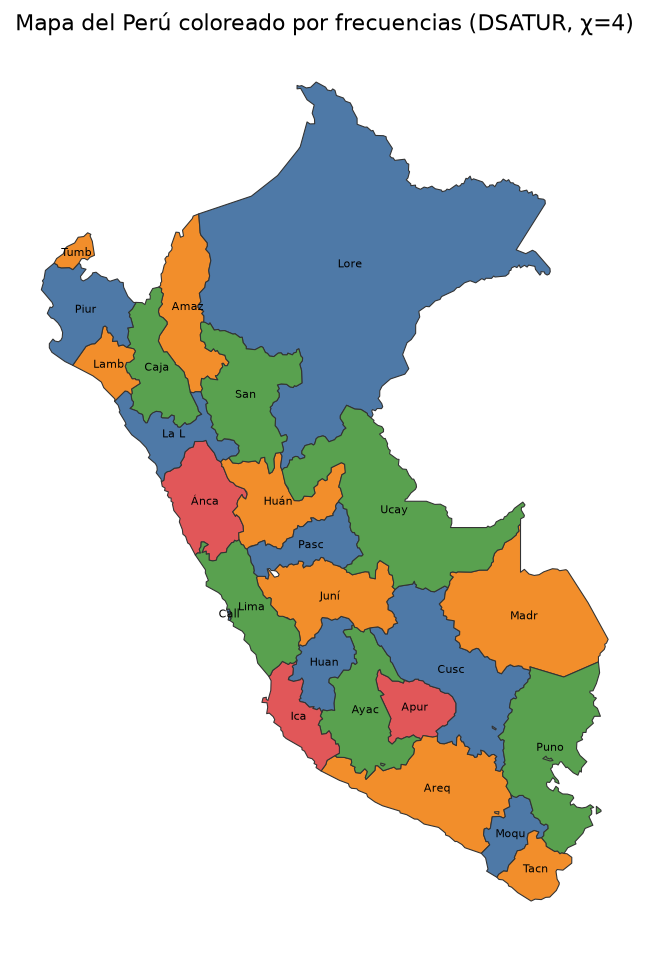
\includegraphics[height=6.4cm]{figs/peru_frecuencias.png}\hfill
  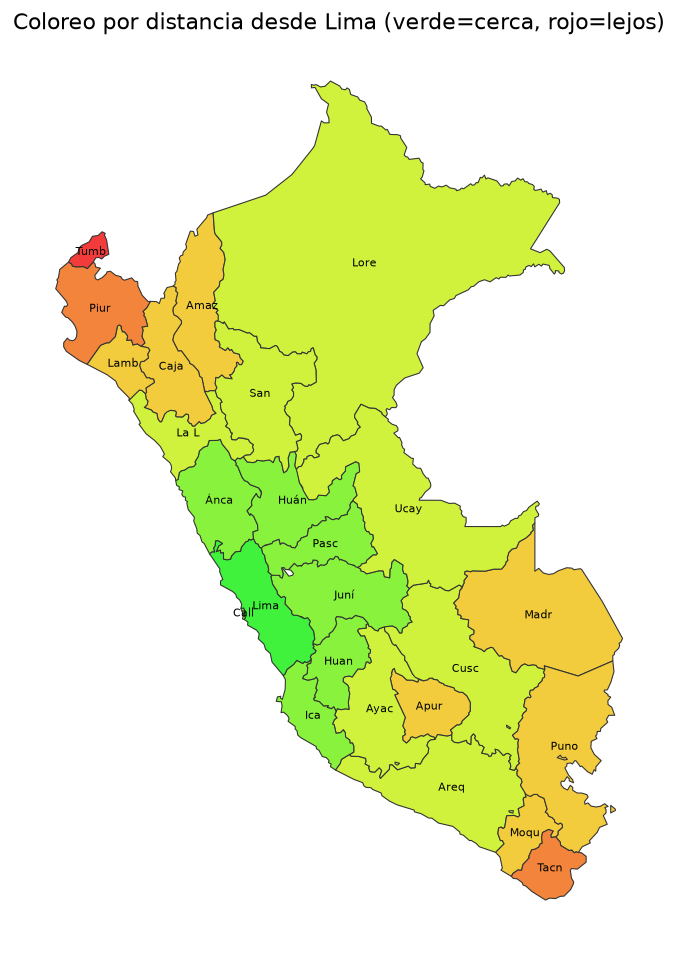
\includegraphics[height=6.4cm]{figs/peru_distancia.png}}{%
  \emph{(Ejecute \texttt{python docs/figuras.py} para generar las figuras.)}}
\caption{Izquierda: coloreo por frecuencias (DSATUR, $\chi=4$). Derecha: coloreo
por distancia (BFS) desde Lima; verde=cerca, rojo=lejos.}\label{fig:mapa}
\end{figure}

\begin{figure}[h]\centering
\IfFileExists{figs/peru_carreteras.png}{%
  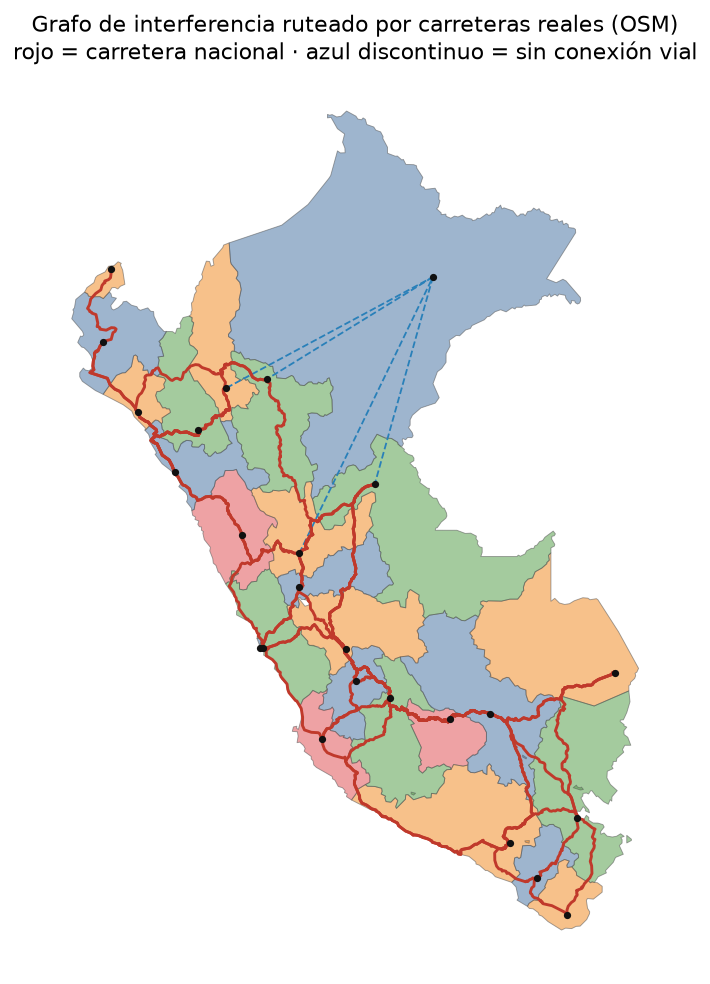
\includegraphics[height=7.2cm]{figs/peru_carreteras.png}}{}
\caption{Grafo de interferencia con las aristas ruteadas sobre la red vial real
(OSM): rojo = carretera nacional; azul discontinuo = par sin conexión vial
(fronteras de Loreto). Los nodos se ubican en las capitales
departamentales.}\label{fig:carreteras}
\end{figure}

En la gráfica log-log (Fig.~\ref{fig:tiempo}) una función $\Theta(n^a)$ es una
recta de pendiente $a$: Greedy y DSATUR sobre grafos geométricos dispersos
($m=\Theta(n)$) siguen la pendiente $1$ de la referencia $\Theta(n)$.

\begin{figure}[h]\centering
\IfFileExists{figs/tiempo_vs_n.png}{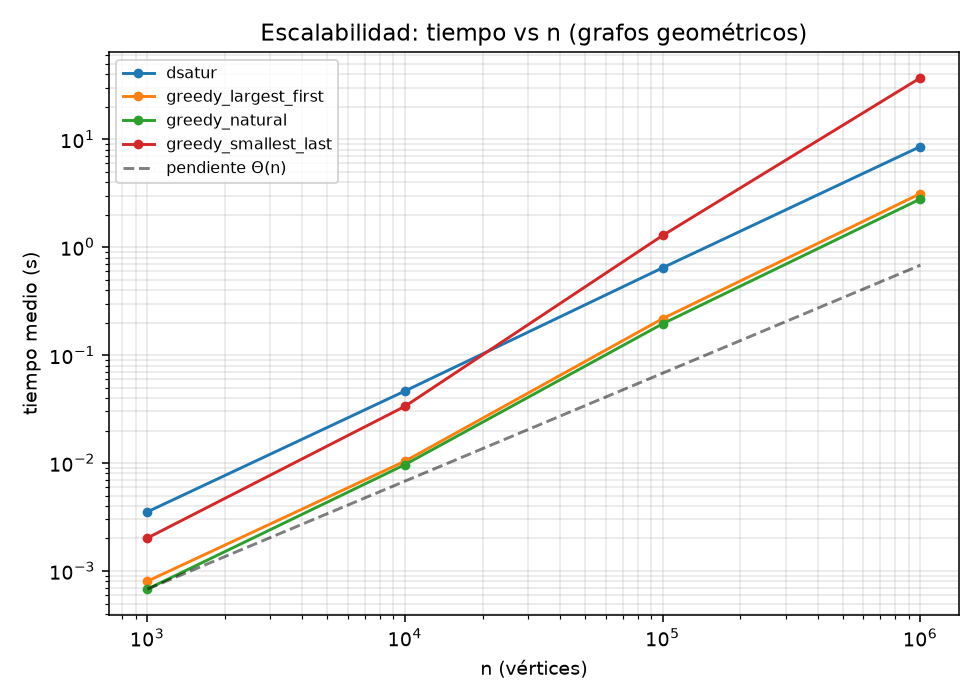
\includegraphics[width=0.7\textwidth]{figs/tiempo_vs_n.png}}{}
\caption{Tiempo medio vs $n$ (log-log). La recta discontinua es $\Theta(n)$.}\label{fig:tiempo}
\end{figure}

\IfFileExists{resultados_tabla.tex}{% Generada por docs/make_tabla.py
\begin{table}[h]\centering\small
\caption{Resultados experimentales (media de repeticiones, semilla 42; backtracking con timeout de 30\,s).}
\begin{tabular}{@{}llrrrrl@{}}
\toprule
\textbf{Instancia} & \textbf{Algoritmo} & $n$ & $m$ & \textbf{Colores} & \textbf{Tiempo} & \textbf{Mem.}\\
\midrule
Peru & Greedy natural & 25 & 53 & 5 & 26\,$\mu$s & 0.00\,MB\\
Peru & Greedy mayor grado & 25 & 53 & 4 & 44\,$\mu$s & 0.00\,MB\\
Peru & Greedy smallest-last & 25 & 53 & 4 & 64\,$\mu$s & 0.01\,MB\\
Peru & DSATUR & 25 & 53 & 4 & 64\,$\mu$s & 0.01\,MB\\
Peru & Backtracking & 25 & 53 & 4 (chi=4 exacto) & 137\,$\mu$s & ---\\
\addlinespace
gnp\_1000 & Greedy natural & 1000 & 4995 & 8 & 957\,$\mu$s & 0.06\,MB\\
gnp\_1000 & Greedy mayor grado & 1000 & 4995 & 7 & 1.38\,ms & 0.06\,MB\\
gnp\_1000 & Greedy smallest-last & 1000 & 4995 & 7 & 2.99\,ms & 0.18\,MB\\
gnp\_1000 & DSATUR & 1000 & 4995 & 5 & 4.16\,ms & 0.64\,MB\\
gnp\_1000 & Backtracking & 1000 & 4995 & 5 (chi en [3) & 30.00\,s & ---\\
\addlinespace
geo\_1000 & Greedy natural & 1000 & 2896 & 9 & 680\,$\mu$s & 0.06\,MB\\
geo\_1000 & Greedy mayor grado & 1000 & 2896 & 9 & 803\,$\mu$s & 0.06\,MB\\
geo\_1000 & Greedy smallest-last & 1000 & 2896 & 9 & 2.02\,ms & 0.14\,MB\\
geo\_1000 & DSATUR & 1000 & 2896 & 9 & 3.53\,ms & 0.44\,MB\\
\addlinespace
geo\_10000 & Greedy natural & 10000 & 30043 & 11 & 9.67\,ms & 0.50\,MB\\
geo\_10000 & Greedy mayor grado & 10000 & 30043 & 10 & 10.40\,ms & 0.51\,MB\\
geo\_10000 & Greedy smallest-last & 10000 & 30043 & 10 & 33.52\,ms & 1.62\,MB\\
geo\_10000 & DSATUR & 10000 & 30043 & 10 & 46.46\,ms & 4.28\,MB\\
\addlinespace
geo\_100000 & Greedy natural & 100000 & 298939 & 12 & 194.93\,ms & 8.26\,MB\\
geo\_100000 & Greedy mayor grado & 100000 & 298939 & 11 & 217.43\,ms & 8.27\,MB\\
geo\_100000 & Greedy smallest-last & 100000 & 298939 & 11 & 1.28\,s & 14.85\,MB\\
geo\_100000 & DSATUR & 100000 & 298939 & 11 & 643.15\,ms & 45.96\,MB\\
\addlinespace
geo\_1000000 & Greedy natural & 1000000 & 2996912 & 13 & 2.78\,s & 67.63\,MB\\
geo\_1000000 & Greedy mayor grado & 1000000 & 2996912 & 13 & 3.12\,s & 68.06\,MB\\
geo\_1000000 & Greedy smallest-last & 1000000 & 2996912 & 13 & 36.92\,s & 124.23\,MB\\
geo\_1000000 & DSATUR & 1000000 & 2996912 & 13 & 8.53\,s & 442.39\,MB\\
\bottomrule
\end{tabular}
\end{table}
}{}

Observaciones: \emph{(i)} en el Perú todos los órdenes salvo el natural alcanzan
$\chi=4$; \emph{(ii)} DSATUR usa menos colores que los greedy en $G(n,p)$ a costa
de más tiempo; \emph{(iii)} el backtracking es exacto e instantáneo en $n=25$
($0$ nodos: las cotas cierran) pero agota su presupuesto en $n=10^3$ ---la
frontera práctica de la exactitud; \emph{(iv)} solo Greedy y DSATUR escalan a
$n=10^6$, coherente con sus cotas casi lineales. En los $n$ grandes,
smallest-last y DSATUR se desvían de la pendiente $1$: no porque su conteo de
operaciones deje de ser lineal (las sumatorias de \S\ref{sec:sl} y
\S\ref{sec:dsatur} lo garantizan), sino porque el costo por operación crece
(cubetas de conjuntos y heap dispersan los accesos a memoria, más el factor
$\log n$ de DSATUR): el modelo RAM de costo uniforme no captura la caché.

% =====================================================================
\section{El caso $n=10^{10}$: por qué es solo teórico}
% =====================================================================
\begin{itemize}[leftmargin=1.6em]
\item \textbf{Memoria}: el arreglo de colores a 2 bytes (\texttt{uint16}) ocupa
  $2\cdot10^{10}$ B $=20$ GB; la adyacencia con grado medio $6$ a 8 bytes,
  $\sim480$ GB. El modelo RAM deja de aplicar (no cabe en memoria).
\item \textbf{Tiempo extrapolado}: la curva medida hasta $10^6$ tiene pendiente
  $\approx1$; escalar $\times10^4$ daría horas \emph{si} la memoria fuera plana,
  pero con paginación a disco domina la E/S.
\item \textbf{Conclusión}: $10^{10}$ es una cota asintótica, no un experimento;
  se aborda con computación distribuida (BSP/Pregel, grafo particionado) o
  memoria externa. El backtracking queda descartado por tiempo exponencial.
\end{itemize}

% =====================================================================
\begin{thebibliography}{9}
\bibitem{clrs} Cormen, Leiserson, Rivest, Stein. \emph{Introduction to
Algorithms}, 4.\textsuperscript{a} ed., MIT Press, 2022.
\bibitem{brelaz} D.~Brélaz. \emph{New methods to color the vertices of a graph}.
CACM 22(4), 1979.
\bibitem{welsh} D.~Welsh, M.~Powell. \emph{An upper bound for the chromatic
number of a graph}. Computer Journal 10(1), 1967.
\bibitem{matula} D.~Matula, L.~Beck. \emph{Smallest-last ordering and clustering
and graph coloring algorithms}. JACM 30(3), 1983.
\bibitem{karp} R.~Karp. \emph{Reducibility among combinatorial problems}, 1972.
\bibitem{bb} V.~Batagelj, U.~Brandes. \emph{Efficient generation of large random
networks}. Phys. Rev. E 71, 036113, 2005.
\bibitem{appel} K.~Appel, W.~Haken. \emph{Every planar map is four colorable}.
Illinois J. Math. 21, 1977.
\end{thebibliography}

\end{document}
